\subsubsubsection*{Propagation Algorithm}
Given the definitions and aproxmations to compute perturbations described in the previous section, a propagation in time for the change in orbital parameters is solved. The results are plotted in the graph below:

\begin{figure}[H]
\centering
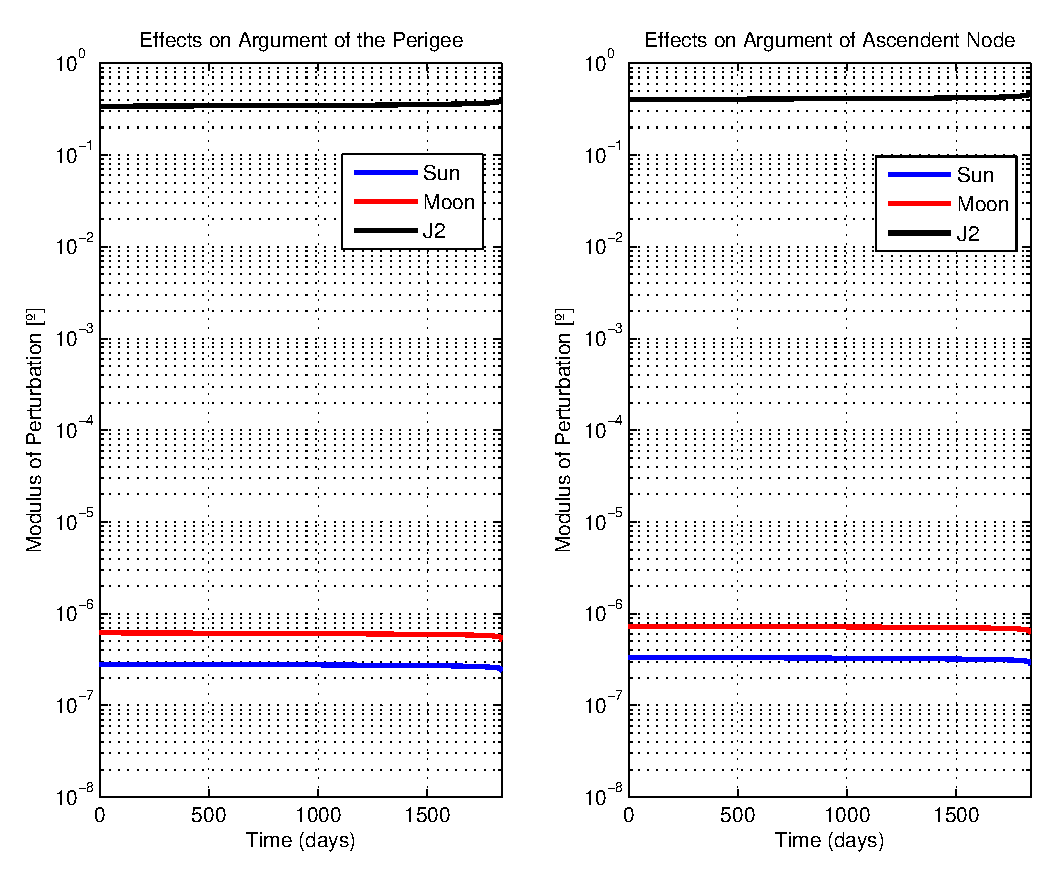
\includegraphics[scale=0.8]{SignificativePerturbations/ModulusAngulars.eps}
\caption{Logaritmic plot of the modulus of the increases in Angular Arguments of the orbit}
\end{figure}

As it can be seen, the perturbations caused by 3rd bodies are several orders of magnitude below the order of magnitude of the variation caused by Earth's oblateness. It is also remarkable that the moon has a higher effect than the sun given the relative distance to Earth, even if the sun is way more massive.

Another important obsevation is that given the very low eccentricity we are considering, the deviation of the argument of the perigee does not affect the performance of the constellation. In other words, since the orbits are considered almost circular there is not a defined Perigee for the orbit.

\subsubsubsection*{In conclusion}
The effects of the Moon and the Sun are neglected in comparison with the effects of J2 for the Argument of the ascendent node as well as for the argument of the Perigee.